\chapter*{Dodatak: Prikaz aktivnosti grupe}
		\addcontentsline{toc}{chapter}{Dodatak: Prikaz aktivnosti grupe}
		
		\section*{Dnevnik sastajanja}
		
		
		\begin{packed_enum}
			\item  sastanak
			
			\item[] \begin{packed_item}
				\item Datum: 20. listopada 2023.
				\item Prisustvovali: F.Sipić, T.Radolović, J.Franjković, J.Vinožganić, T.Matošević, F.Bernt, M.Bolt
				\item Teme sastanka:
				\begin{packed_item}
					\item  inicijalni dogovor o temi projekta
					\item  prijedlozi tehnologija i arhitekture
				\end{packed_item}
			\end{packed_item}
			
			\item  sastanak
			\item[] \begin{packed_item}
				\item Datum: 2. studenoga 2023.
				\item Prisustvovali: F.Sipić, T.Radolović, J.Franjković, J.Vinožganić, T.Matošević, F.Bernt, M.Bolt
				\item Teme sastanka:
				\begin{packed_item}
					\item  podjela u podtimove, frontend, backend, dokumentacija
				\end{packed_item}
			\end{packed_item}

			\item  sastanak
			\item[] \begin{packed_item}
				\item Datum: 4. studenoga 2023.
				\item Prisustvovali: F.Sipić, T.Radolović, J.Franjković, J.Vinožganić, T.Matošević, F.Bernt, M.Bolt
				\item Teme sastanka:
				\begin{packed_item}
					\item  dogovor o strukturi baze podataka
				\end{packed_item}
			\end{packed_item}

			\item  sastanak
			\item[] \begin{packed_item}
				\item Datum: 6. studenoga 2023.
				\item Prisustvovali: F.Sipić, T.Radolović, J.Franjković, J.Vinožganić, T.Matošević, F.Bernt, M.Bolt
				\item Teme sastanka:
				\begin{packed_item}
					\item  podjela zadataka za sljedeći tjedan
				\end{packed_item}
			\end{packed_item}

			\item  sastanak
			\item[] \begin{packed_item}
				\item Datum: 8. studenoga 2023.
				\item Prisustvovali: F.Sipić, J.Franjković, J.Vinožganić, M.Bolt
				\item Teme sastanka:
				\begin{packed_item}
					\item  dogovor o postavljanju backend okruženja
				\end{packed_item}
			\end{packed_item}

			\item  sastanak
			\item[] \begin{packed_item}
				\item Datum: 9. studenoga 2023.
				\item Prisustvovali: F.Bernt, T.Radolović, T.Matošević, M.Bolt
				\item Teme sastanka:
				\begin{packed_item}
					\item  dogovor o postavljanju frontend okruženja
				\end{packed_item}
			\end{packed_item}

			\item  sastanak
			\item[] \begin{packed_item}
				\item Datum: 14. studenoga 2023.
				\item Prisustvovali: F.Sipić, J.Franjković, J.Vinožganić, M.Bolt, T.Radolović, T.Matošević, F.Bernt
				\item Teme sastanka:
				\begin{packed_item}
					\item  dogovor o deploymentu aplikacije
				\end{packed_item}
			\end{packed_item}

			\item  sastanak
			\item[] \begin{packed_item}
				\item Datum: 5. prosinca 2023.
				\item Prisustvovali: F.Sipić, J.Franjković, J.Vinožganić, M.Bolt, T.Radolović, T.Matošević, F.Bernt
				\item Teme sastanka:
				\begin{packed_item}
					\item  dogovor o nastavku razvoja aplikacije
					\item podjela zadataka za sljedećih nekoliko tjedana
				\end{packed_item}
			\end{packed_item}

			\item  sastanak
			\item[] \begin{packed_item}
				\item Datum: 20. prosinca 2023.
				\item Prisustvovali: F.Sipić, J.Franjković, F.Bernt
				\item Teme sastanka:
				\begin{packed_item}
					\item  pregled i ispravljanje grešaka u dokumentaciji
				\end{packed_item}
			\end{packed_item}
			
			\item  sastanak
			\item[] \begin{packed_item}
				\item Datum: 14. siječnja 2024.
				\item Prisustvovali: F.Sipić, J.Franjković, F.Bernt, J. Vinožganić, T. Radolović, T. Matošević, M. Bolt
				\item Teme sastanka:
				\begin{packed_item}
					\item  finalni sastanak za završnu predaju, ispravke dokumentacije i koda
				\end{packed_item}
			\end{packed_item}
			
			%
			
		\end{packed_enum}
		
		\eject
		\section*{Tablica aktivnosti}
		
			\textbf{\textit{Kontinuirano osvježavanje}}\\
			
			 \textit{Napomena: Doprinose u aktivnostima treba navesti u satima po članovima grupe po aktivnosti.}

			\begin{longtblr}[
					label=none,
				]{
					vlines,hlines,
					width = \textwidth,
					colspec={X[7, l]X[1, c]X[1, c]X[1, c]X[1, c]X[1, c]X[1, c]X[1, c]}, 
					vline{1} = {1}{text=\clap{}},
					hline{1} = {1}{text=\clap{}},
					rowhead = 1,
				} 
			
				\SetCell[c=1]{c}{} & \SetCell[c=1]{c}{\rotatebox{90}{\textbf{Marko Bolt}}} & \SetCell[c=1]{c}{\rotatebox{90}{\textbf{Filip Bernt }}} &	\SetCell[c=1]{c}{\rotatebox{90}{\textbf{Teo Matošević }}} & \SetCell[c=1]{c}{\rotatebox{90}{\textbf{Teo Radolović }}} &	\SetCell[c=1]{c}{\rotatebox{90}{\textbf{Jure Franjković }}} & \SetCell[c=1]{c}{\rotatebox{90}{\textbf{Fran Sipić }}} &	\SetCell[c=1]{c}{\rotatebox{90}{\textbf{Jakov Vinožganić }}} \\  
				Upravljanje projektom 		& 10 &  & 4 &  &  &  & 3 \\ 
				Opis projektnog zadatka 	& 3 &  &  &  &  &  & \\ 
				
				Funkcionalni zahtjevi       &  &  &  & 3 &  & 2  & 4 \\ 
				Opis pojedinih obrazaca 	&  & 2 &  &  &  &  &  \\ 
				Dijagram obrazaca 			&  & 5 &  &  &  &  &  \\
				Sekvencijski dijagrami 		&  &  & 1 &  &  & 6 &  \\ 
				Opis ostalih zahtjeva 		&  &  &  &  & 3 &  &  \\ 

				Arhitektura i dizajn sustava	 &  &  &  &  & 3 &  &  \\ 
				Baza podataka				&  & 1 &  &  &  & 4 &   \\ 
				Dijagram razreda 			&  &  &  &  & 6 &  &   \\ 
				Dijagram stanja				&  &  &  &  &  &  3  \\ 
				Dijagram aktivnosti 		&  &  &  &  & 3 &  &  \\ 
				Dijagram komponenti			&  & 3 &  &  &  &  &  \\ 
				Korištene tehnologije i alati 		&  &  &  &  & 1 &  &  \\ 
				Ispitivanje programskog rješenja 	& 2 & 3 &  &  & 3 & 6 &  \\ 
				Dijagram razmještaja			&  &  &  &  &  & 3 &  \\ 

				Upute za puštanje u pogon 		&  & 2 &  &  &  &  &  \\  
				Dnevnik sastajanja 			&  &  &  &  &  & 2 &  \\ 

				Zaključak i budući rad 		& 2 &  &  &  &  &  &  \\  
				Popis literature 			&  & 1 &  &  &  &  &  \\   
				\textit{Dodatne stavke kako ste podijelili izradu aplikacije} 			&  &  &  &  &  &  &  \\ 
				\textit{front end} 				& 10 & 15 & 15 & 20 &  & 10 & 30 \\  
				\textit{izrada baze podataka} 		 			& 2  &  & 3 &  &  &  & 4\\  
				\textit{spajanje s bazom podataka} 							& 2 &  &  &  &  &  & 2 \\ 
				\textit{back end} 							& 4 &  &  &  & 6 & 10 & 10 \\ 
				\textit{deploy} 							& 8 &  & 2 & 6 &  &  &  \\ 
				 						 
			\end{longtblr}
					
					
		\eject
		\section*{Dijagrami pregleda promjena}
		
		\noindent Na prikazanim grafovima se nalaze samo promjene grane development na svim repozitorijima, te neki članovi nisu imali podudarajuće e-mailove na lokalnom računalu i GitHub-u zato se ne prikazuju kao \textit{Contributors}. Također se ne prikazuje aktivnost na svim granama već samo na development jer GitHub ne nudi opciju prikaza aktivnosti ostalih grana. \\
		\newline \noindent Popis commitova preostalih članova grupe:
		\begin{packed_item}
			\item Jakov Vinožganić - \textbf{84 commitova}
			\item Fran Sipić - \textbf{30 commitova}
		\end{packed_item}
		\noindent Prikaz pregleda promjena na svim repozitorijima:
		\begin{packed_enum}
			\item \textbf{bytepit-ui}
			
			\begin{figure}[H]
				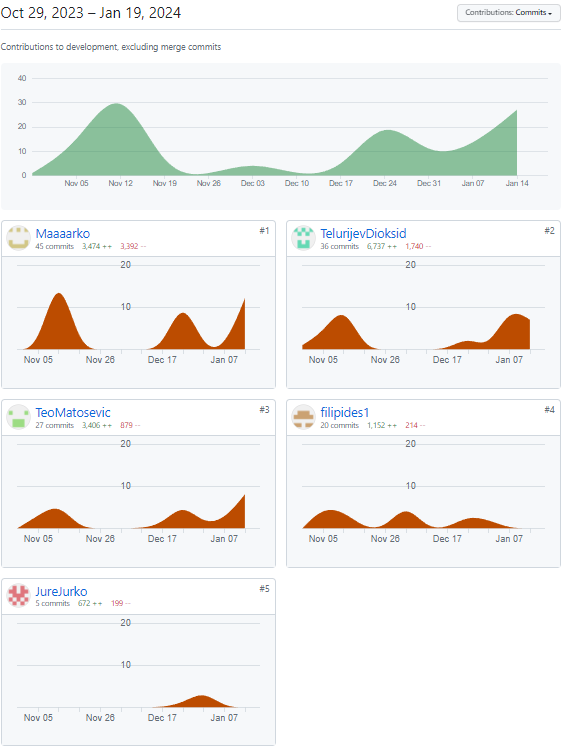
\includegraphics[scale=0.75]{slike/bp-ui-contr.PNG} 
				\centering
				\caption{Bytepit-ui}
				\label{fig:bytepit-ui}
			\end{figure}
			
			\eject
			
			\item \textbf{bytepit-api}
			
			\begin{figure}[H]
				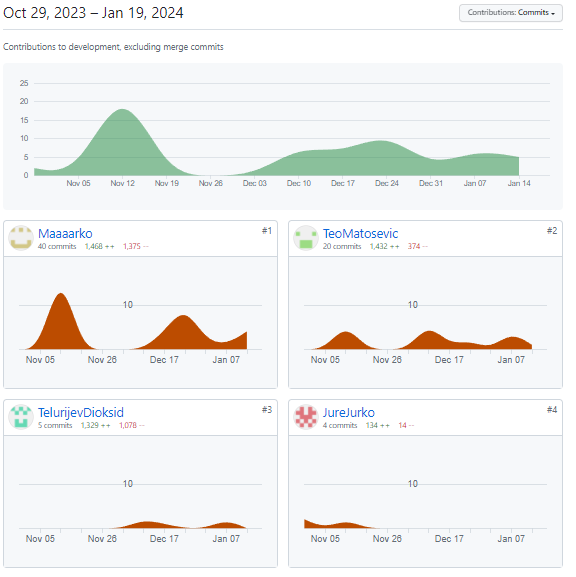
\includegraphics[scale=1.0]{slike/bp-api-contr.PNG} 
				\centering
				\caption{Bytepit-api}
				\label{fig:bytepit-api}
			\end{figure}
			
			\eject
			
			\item \textbf{bytepit-root}
			
			\begin{figure}[H]
				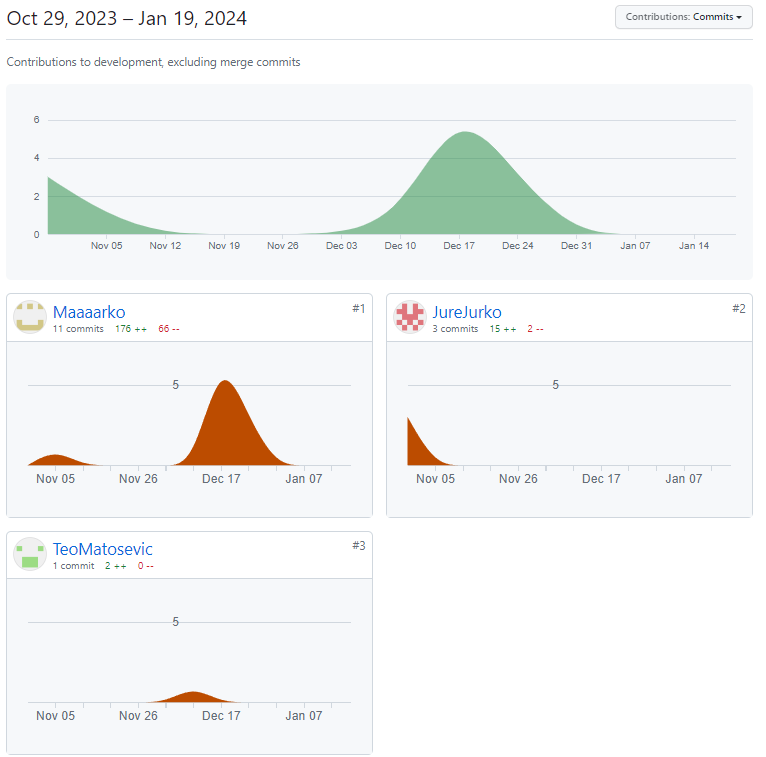
\includegraphics[scale=0.9]{slike/bp-root-contr.PNG} 
				\centering
				\caption{Bytepit-root}
				\label{fig:bytepit-root}
			\end{figure}
		\end{packed_enum}
		
		  
		
	